\documentclass[titlepage,10pt,a4paper]{article}
\usepackage[utf8]{inputenc}
\usepackage{graphicx}
\usepackage{hyperref}
\usepackage[ngerman]{babel}
\usepackage{float}
\usepackage{subcaption}
\usepackage{listings}
\usepackage{color}

\usepackage{glossaries}
\makeglossaries

\newglossaryentry{Server}{name={Server},
description={Der zentral ausgeführte Teil der Software, der die Kommunikation und
Interaktion mit den Clients verwaltet sowie erstellte Spiele verwaltet und
die Einhaltung der Regeln in diesen gewährleistet. }}

\newglossaryentry{Erstellungsfenster}{name={Erstellungsfenster},
description={Fenster in welchem der Spielleiter die Eigenschaften des Spiels festlegt}}

\newglossaryentry{Lobby}{name={Lobby},
description={Ort, an dem Spieler ein neues Spiel erstellen oder einem Spiel beitreten können}}

\newglossaryentry{Regelwerk}{name={Regelwerk},
description={Ein bestimmtes Kartenspiel, bzw. die Regeln und Eigenschaften von diesem}}

\newglossaryentry{Spielleiter}{name={Spielleiter},
description={Derjenige, der das Spiel erstellt hat}}

\newglossaryentry{Wartefenster}{name={Wartefenster},
description={Fenster in welchem man sich befndet, während man darauf wartet, dass die Mindestteilemerzahl erfüllt ist und das Spiel gestartet wird}}

\newglossaryentry{IP-Adresse}{name={IP-Adresse},
description={}}

\title{Handbuch}
\date{\today{}, Passau}

\begin{document}
\begin{titlepage}
\vspace*{3cm}
\begin{center}
\textbf{\textsc{\LARGE Handbuch}}

{\large \today}

\vspace{2cm}
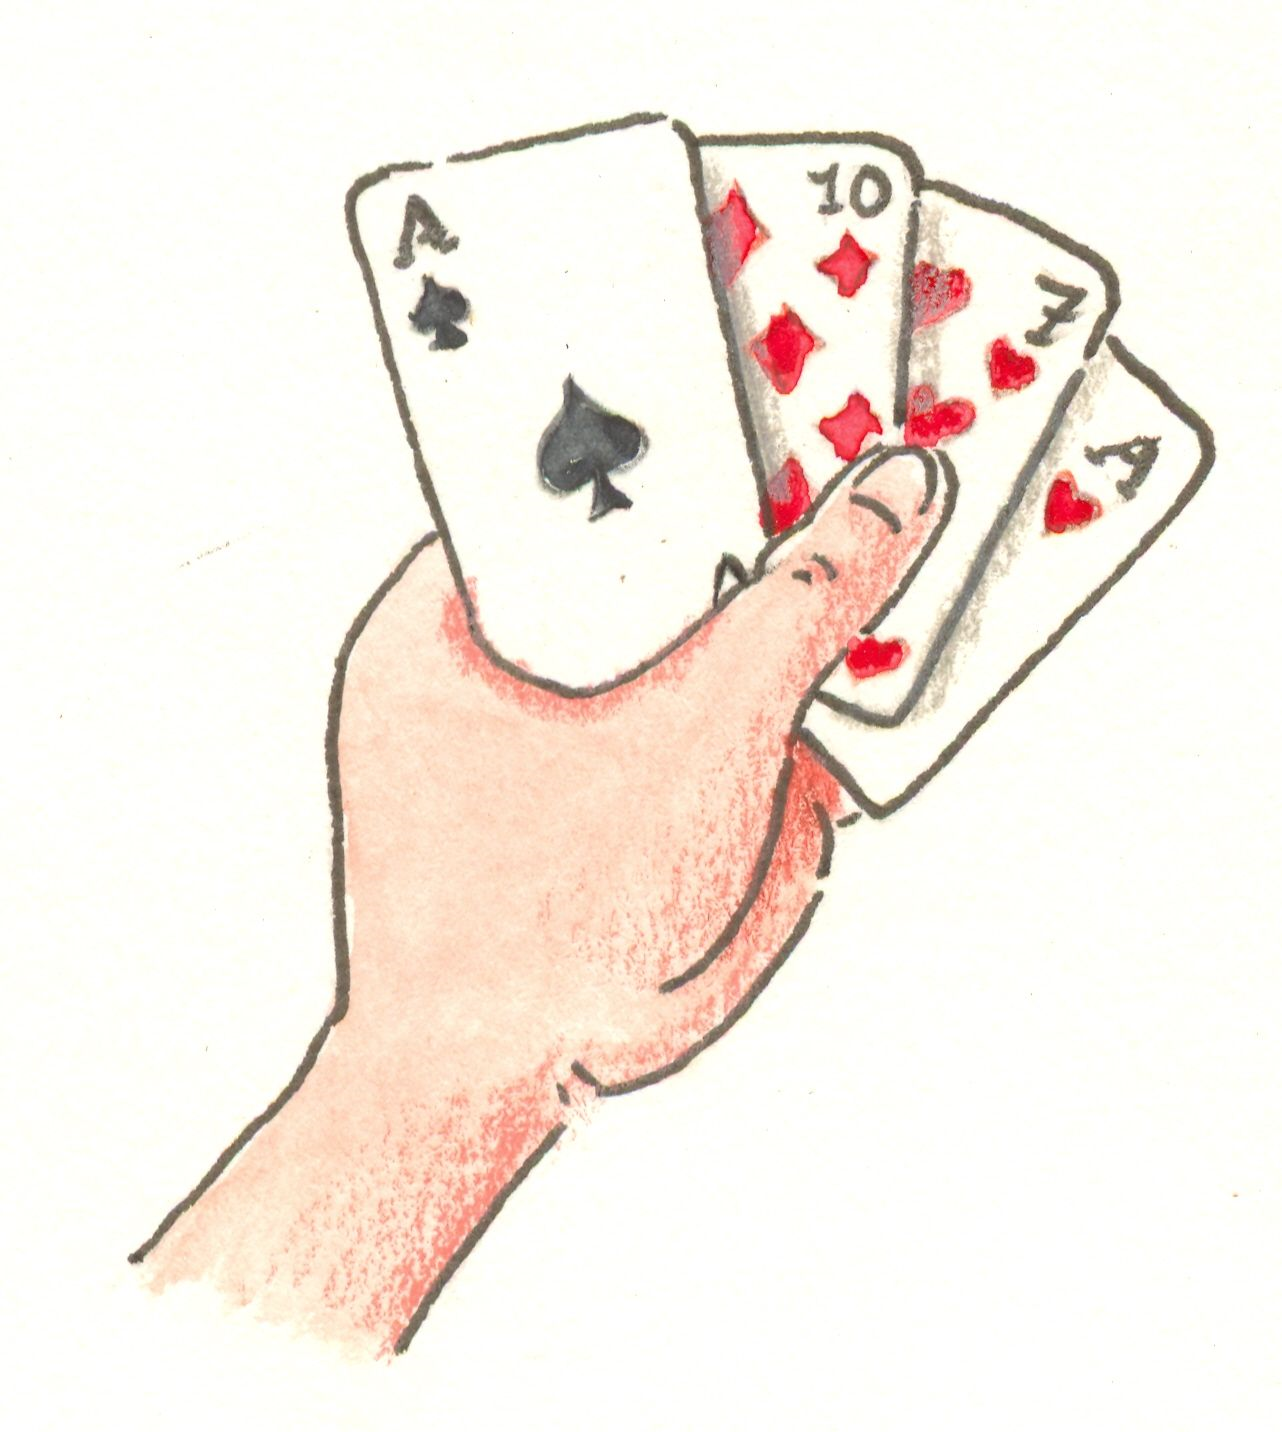
\includegraphics{kartenspiel}
\ \\
\ \\

\textbf{\textsc{\LARGE NET-WizHearts}}
\vspace{2cm}

\begin{tabular}{|c|c|c|}\hline
   Phase & Verantwortlicher & E-Mail \\ \hline\hline
   Pflichtenheft & Alina Meixl &  alina@meixl.de \\ \hline
   Entwurf & Viktoria Witka & witkaviktoria@freenet.de \\ \hline
   Spezifikation & Daniel Riedl & dariedl14@yahoo.de \\ \hline
   Implementation & Andreas Altenbuchner& a.andi007@gmail.com\\ \hline
   Verifikation & Patrick Kubin & kubin@fim.uni-passau.de\\ \hline
   Präsentation & w& w\\ \hline
 \end{tabular}
\vspace{2cm}
\\
\end{center}
\end{titlepage}
\tableofcontents
\pagenumbering{arabic}
\hypersetup{pageanchor=true}

\newpage
 
\section{Einleitung}
Dies ist das Handbuch zum Spiel NET-WizHearts. NET-WizHearts ist ein Mulitplayer-Online-Kartenspielsystem, durch das mehrere Spieler über das Internet gegeneinander spielen können. Es gibt verschiedene Regelwerke, die gespielt werden können. Mitgeliefert werden bereits Hearts und Wizard. Die Anwendung ist so konzipiert, dass jederzeit weitere \gls{Regelwerk}e hinzugefügt werden können.

\section{Systemvoraussetzungen}
Dieses Produkt läuft auf den Betriebssystemen Microsoft Windows, Mac OS X und Linux. Java 7 Laufzeitumgebung muss vorhanden sein. Für das Spielen online ist ausserdem eine Internetverbindung vonnöten. \\
\gls{Server}seitig müssen zusätzlich die Mindestanforderungen des verwendeten Betriebssystems bezüglich Arbeitsspeicher und Rechenleistung erfüllt sein. Diese können durch die Anzahl der gehosteten Spieler/Spiele steigen.

\section{Installation}

\section{Haftungsausschluss}

\section{Spiel}
\subsection{Einloggen}
Sobald Sie die Anwendung starten, sehen Sie als erstes das Login-Fenster. In diesem Fenster ein können Sie sich mit einem Benutzernamen anmelden und zu einem \gls{Server}r verbinden. Außerdem können Sie auswählen, in welcher Sprache das Programm laufen soll.\\
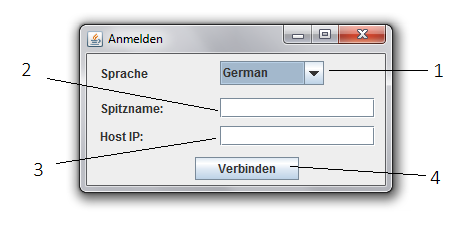
\includegraphics[width=\textwidth]{Login-Fenster}
\begin{itemize}
	\item \textbf{1) Sprachauswahl:} Hier können Sie in einem Dropdown-Menü aus den Sprachen Deutsch, Englisch und Bayerisch wählen.
	\item \textbf{2) Eingabefeld für den Benutzernamen:} Hier geben Sie Ihren Benutzernamen ein. Dieser muss Eindeutig sein, sollte bereits ein anderer Spieler diesen Namen gewählt haben, werden Sie dazu aufgefördert, einen anderen Namen zu wählen
	\item \textbf{3) Eingabefeld für die \gls{IP-Adresse} des \gls{Server}s:} In dieses Feld geben Sie die\gls{IP-Adresse} des \gls{Server}s ein, zu dem Sie sich vebinden möchten
	\item \textbf{4) Verbindungsknopf:} Wenn Sie auf diesen Knopf drücken, wird die Verbindung zum \gls{Server} hergestellt, und Sie betreten die \gls{Lobby} (siehe Kap. 5.2)
\end{itemize}

\subsection{Spiel betreten}
In der \gls{Lobby} können Sie ein Spiel erstellen, oder einem existierenden Spiel beitreten. Das Chatten mit anderen Mitspielern in der \gls{Lobby} ist möglich.\\
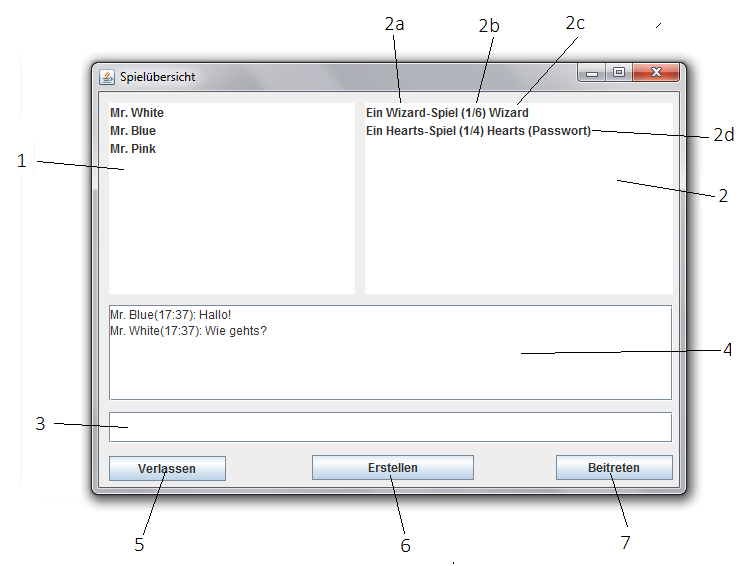
\includegraphics[width=\textwidth]{Lobby-Fenster}
\begin{itemize}
	\item \textbf{1) Spielerliste:} Hier sehen Sie Benutzernamen aller Spieler, die sich momentan in der \gls{Lobby}v befinden
	\item \textbf{2) Spielliste:} Hier sehen Sie alle Spiele, die momentan noch auf Mitspieler warten oder noch nicht gestartet sind
	\begin{itemize}
		\item \textbf{2a) Spielname:} Der Name des Spieles
		\item \textbf{2b) Spielerzahl:} Die Anzahl der momentanen Spieler/Die Anzahl der maximalen Spieler
		\item \textbf{2c) Regelwerk:} Welche  Art von Spiel gespielt wird
		\item \textbf{2d) Passwort:} Zeigt an, ob der Beitritt zum Spiel Passwortgeschüzt ist
	\end{itemize}
	\item \textbf{3) Eingabefeld für den Chat:} In dieses Feld geben Sie ihre Chatnachrichten ein. Mit ENTER werden Sie versendet.
	\item \textbf{4) Chatverlauf:} Hier sehen Sie Ihre Chatnachrichten und die der anderen Nutzer
	\item \textbf{5) Verlassen-Knopf:} Wenn Sie diesen Knopf drücken, wird die Anwendung beendet
	\item \textbf{6) Erstellen-Knopf:} Drücken Sie diesen Knopf, wenn Sie ein neues Spiel erstellen wollen (mehr dazu in Kap. 5.3)
	\item \textbf{7) Beitreten-Knopf:} Wählen Sie ein Spiel in der Spieliste aus und drücken Sie auf diesen Knopf, um dem Spiel beizutreten. Ist das Spiel Passwortgeschützt, erscheint folgendes Fenster, in welches Sie das Passwort eingeben müssen, um in die \gls{Wartefenster} zu gelangen.
\end{itemize}
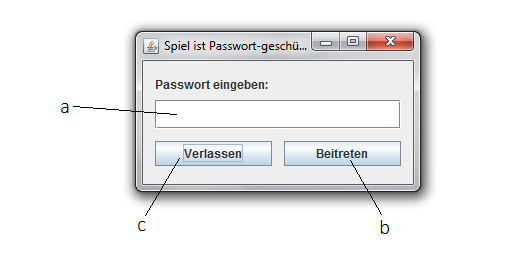
\includegraphics[width=\textwidth]{Passwort-Fenster}
\begin{itemize}
		\item \textbf{a) Passworteingabe:} Hier geben Sie das Passwort für das geschützte Spiel ein. Sollte es nicht mit dem gesetzten Passwort übereinstimmen, erhalten Sie eine Warnmeldung.
		\item \textbf{b) Beitreten-Knopf:} Drücken Sie auf diesen Knopf um das Passwort überprüfen zu lassen und dem Spiel beizutreten. Bei korrektem Passwort betreten Sie das \gls{Wartefenster} (siehe Kap. 5.3)
		\item \textbf{c) Verlassen-Knopf:} Die Texteingabe wird abgebrochen und Sie kehren in die \gls{Lobby} zurück
\end{itemize}

\subsection{Spiel erstellen}
In der Lobby können Sie ein neues Spiel erstellen indem Sie auf den Erstellen-Knopf (6)  drücken. Sie kommen in das \gls{Erstellungsfenster}.\\
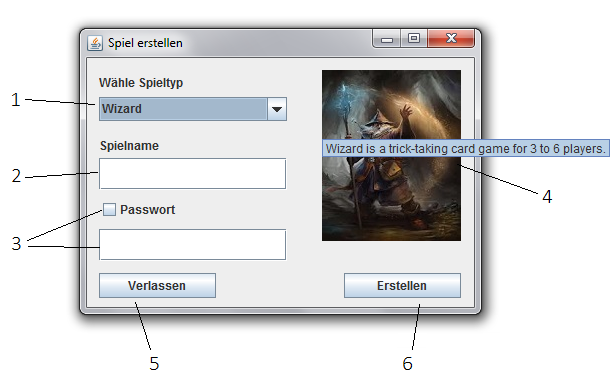
\includegraphics[width=\textwidth]{Erstellungs-Fenster}
\begin{itemize}
	\item \textbf{1) Spielauswahl:} Hier können Sie in einem Dropdown-Menü aus den\gls{Regelwerk}en Hearts oder Wizard auswählen
	\item \textbf{2) Eingabefeld für den Spielnamen:} Hier können Sie Ihrem Spiel einen Namen geben. Lassen Sie das Feld frei, so wird ein Standard Name für das Spiel gesetzt, bestehend aus Ihrem Benutzernamen + 's Spiel'.
	\item \textbf{3) Passwortschutz:} Wenn Sie in dem oberen Feld ein Häckchen setzen, können Sie den Zutritt zu Ihrem Spiel mit einem Passwort schützen, welches Sie in das untere Feld eingeben
	\item \textbf{4) Spielbild:} Ein Bild passend zum\gls{Regelwerk}, welches Sie ausgewählt haben. Wenn Sie mit der Maus über das Bild fahren, erscheint eine Kurzbeschreibung zu diesem Spiel.
	\item \textbf{5) Verlassen-Knopf:} Wenn Sie diesen Knopf drücken, wird die Spielerstellung abgebrochen, und Sie kommen in die Lobby zurück
	\item \textbf{6) Erstellen-Knopf:} Wenn Sie mit Ihren Einstellungen Fertig sind, drücken Sie auf diesen Knopf, um das Spiel zu erstellen. Sie betreten das \gls{Wartefenster} wo Sie auf den Beitritt von weiteren Spielern warten müssen, bis die Mindestzahl der Spieler erreicht ist, um das Spiel endgültig zu starten.	
\end{itemize}
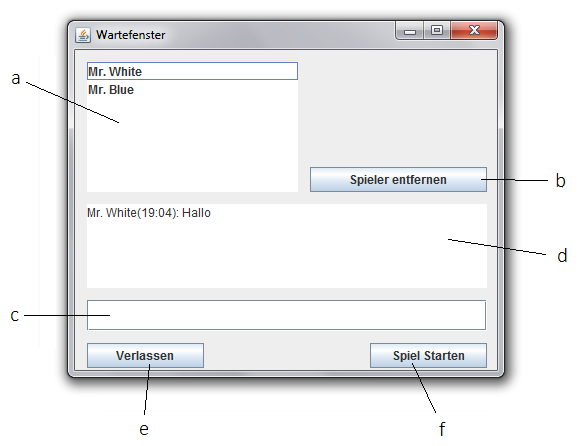
\includegraphics[width=\textwidth]{Warte-Fenster}
\begin{itemize}
	\item \textbf{a) Spielerliste:} Hier sehen Sie Benutzernamen aller Spieler, die sich momentan im \gls{Wartefenster} befinden
	\item \textbf{b) Entfernen-Knopf:} Dieser Knopf ist nur für den Spielleiter sichtbar. Sie können damit andere Spieler aus dem \gls{Wartefenster} entfernen, die daraufhin wieder in die \gls{Lobby} zurückkehren. (Sie können sich nicht selbst aus dem \gls{Wartefenster} werfen. Bitte verbenden Sie den Verlassen-Knopf, wenn Sie in die \gls{Lobby} zurück möchten.)
	\item \textbf{c) Eingabefeld für den Chat:} In dieses Feld geben Sie ihre Chatnachrichten ein. Mit ENTER werden Sie versendet.
	\item \textbf{d) Chatverlauf:} Hier sehen Sie Ihre Chatnachrichten und die der anderen Nutzer
	\item \textbf{e) Verlassen-Knopf:} Mit diesem Knopf kehren Sie in die \gls{Lobby} zurück. Sollte der \gls{Spielleiter} das \gls{Wartefenster} verlassen, so wird das Spiel aufgelöst und alle Spieler werden an die Lobby zurück geschickt.
	\item \textbf{f) Start-Knopf:} Dieser Knopf ist nur für den \gls{Spielleiter} sichtbar. Sobald die Mindestanzahl an Spielern erreicht ist, kann damit das Spiel gestartet werden und das Spielfenster öffnet sich. (siehe Kap. 5.4)
\end{itemize}

\subsection{Spiel spielen}
Nachdem das Spiel im \gls{Wartefenster} gestartet wurde, befinden Sie sich nun im Spielfenster.
\subsubsection{Wizard}
\subsubsection{Hearts}

\section{Fehlermeldungen und Behebung}

\section{Entwicklung eines neuen \gls{Regelwerk}es}
   
\printglossaries

\end{document}